\chapter{Used algorithms}

In previous chapter you have been familiarized with several kinds of agents, how they can be used and also what a spatial memory is. I have briefly prepaired you for the next chapters, where I will explain my contribution to this area. This chapter is going to cover the used algorithms and computational methods I have studied and implemented in my work. 

The first subsection disserts on the implementations of agents' memory and in detail describes fundamental parts. Both the Growing Neural Gas and the Quad..blah are used as memory storages to handle spatial information about the environment with bounded resources.

\section{Growing Neural Gas}

\subsection{Topology learning}

Processing an enormous spatial data about an environment is computationaly demanding when for example we want to navigate in that environment. A topology learning or recognition can help us to create a representation such as topological map which can be viewed as a graph and which makes reasoning in that environment much easier. Rather complex understanding of topology in an indoor space using Bayesian programming has been shown in \cite{Tapus:topologylearning}. It goes much farther than I need to. 

Based on competitive Hebbian learning (CHL) method \cite{Martinetz:chl} and Neural Gas (NG) \cite{Martinetz:ng} Bern Fritzke suggested earlier mentioned Growing Neural Gas \cite{Fritzke:gng}, an unsupervised learning method for finding a topological structure which reflects the topology of the data distribution. Although the combination of both CHL and NG is an effective method for topology learning, there are some flaws in practical application as it requires an initial setup of number of nodes/centers that are used. This fact prevents the method from adequately describing the topology, when a different number of nodes would work better.

As Fritzke described the algorithm uses a set of nodes and edges that connects the nodes. A simplified describtion of algorithm in context of two-dimensional space follows:

\begin{enumerate}
\item Add two nodes at random position onto canvas
\item Generate input signal based on the data distribution (its probability density)
\item Find the nearest node $n_1$ and second nearest node $n_2$ to the signal
\item Increment the age of all edges leading from node $n_2$
\item Moved node $n_1$ and its topological neighbors towards the signal (according to parametres $epsilon_{winner}$ and $epsilon_{neighbour}$)
\item Remove all edges with an age larger than $a_{max}$
\item Generate new nodes
\item Go to 1.
\end{enumerate}

For the purpose of this work I want to use this algorithm to learn a topology of data which dynamically changes through the time. In following subsection I am going to introduce you to the experimenting with this algorithm.

\subsection{Experiments on dynamic data}

\section{Quad}

The idea for this data structure representing resource-bounded memory is based on \cite{Brom:placeandobjects}. What differs in my work from their observed environment is agents in my simulation act in a homogeneous space which cannot be differentiated in a way the mentioned simulation does. To solve this issue I have found inspiration in Quad-tree structures \cite{Finkel:quadtrees} which are used, among others, for storaging more dimensional objects.

\begin{definition}The {\bf quadtree} is a tree structure where each node has exaclty four children. 
\end{definition}
                  
In \ref{usedalgorithms:qtc} and \ref{usedalgorithms:qtc} you can se an example how is a two-dimensional object such as a circle is stored in quadtree.               
                  
\begin{figure}
  \centering                                      
  \includegraphics[scale=1]{diagrams/usedalgorithms/quadtree-circle.eps} 
  \caption{Example of a circle in two-dimensional space}      
  \label{usedalgorithms:qtc}
\end{figure}

\begin{figure}
  \centering                                
  \includegraphics[scale=.8]{diagrams/usedalgorithms/quadtree-treeview.eps} 
  \caption{Quadtree structure of \ref{usedalgorithms:qtc}}
  \label{usedalgorithms:qttv}
\end{figure}
 
Similary I will use this structure to keep spatial information about the environment in the simulation.
